% ClearEval -- IEEE BIBM submission (converted from the MICCAI 2026 LNCS manuscript)
% Two-column IEEE conference format (IEEEtran). Content maps the MICCAI
% manuscript section-by-section; structure/numbers/claims are preserved.
% Compile: pdflatex main -> bibtex main -> pdflatex main -> pdflatex main

\documentclass[conference]{IEEEtran}
\IEEEoverridecommandlockouts
% The preceding line is only needed to identify funding in the first footnote.
% If that is unneeded, please comment it out.

\usepackage{cite}
\usepackage{amsmath,amssymb,amsfonts}
\usepackage{graphicx}
\usepackage{booktabs}
\usepackage{multirow}
\usepackage{textcomp}
\usepackage{xcolor}
\usepackage[T1]{fontenc}
\usepackage{url}
\usepackage{tabularx}
\usepackage{booktabs}
\usepackage{tabularx}


\begin{document}

\title{ClearEval: A Database-Grounded Feasibility Benchmark for LLM-Generated Tissue Optical Clearing Protocols}

% ---------------------------------------------------------------------------
% NOTE: IEEE BIBM uses double-blind review. The author block below is
% anonymized to mirror the MICCAI submission. For the camera-ready version,
% delete the anonymized block and uncomment the six-author IEEE template.
% ---------------------------------------------------------------------------
\author{\IEEEauthorblockN{Anonymous Author(s)}
\IEEEauthorblockA{\textit{Affiliation withheld for double-blind review} \\
email withheld}}

% --- Camera-ready author template (IEEEtran supports up to six authors) ---
% \author{\IEEEauthorblockN{1\textsuperscript{st} Given Name Surname}
% \IEEEauthorblockA{\textit{dept. name of organization (of Aff.)} \\
% \textit{name of organization (of Aff.)}\\
% City, Country \\
% email address or ORCID}
% \and
% \IEEEauthorblockN{2\textsuperscript{nd} Given Name Surname}
% \IEEEauthorblockA{\textit{dept. name of organization (of Aff.)} \\
% \textit{name of organization (of Aff.)}\\
% City, Country \\
% email address or ORCID}
% }

\maketitle

\begin{abstract}
Tissue Optical Clearing (TOC) enables non-destructive, high-resolution 3D
imaging, but protocol design requires compatible choices of clearing method,
labeling strategy, refractive-index condition, and incubation time. While LLMs
perform well on biomedical knowledge tasks, their ability to generate feasible
wet-lab protocols remains under-evaluated. We introduce ClearEval, a
database-grounded feasibility benchmark for LLM-generated TOC protocols.
ClearEval is built on a structured TOC feasibility database integrating 372
wet-lab experimental records, 400+ curated tissue-clearing literature chunks,
and expert-reviewed constraints on methods, tissues, markers, timing, and
compatibility. It evaluates 13 state-of-the-art LLMs through two tracks: 2{,}588
multiple-choice questions for static knowledge and 253 open-ended scenarios for
protocol generation. Generated protocols are scored by our Completeness,
Correctness, and Effectiveness (CCE) framework, which combines rubric-based
procedural assessment with database-grounded feasibility rules and formulas.
Models achieve 79--91\% on the Knowledge Index, but performance drops sharply
for executable protocol generation---for example, GPT-5.2-Fast achieves 91.1\%
on the Knowledge Index but only 61.2 on the Application Index. The main
failures arise from executable parameterization, especially matching fluorescent
markers to required labeling targets. ClearEval provides a depth-first TOC
feasibility benchmark and a re-curatable CCE recipe for related wet-lab
subdomains. Code and data:
\url{https://anonymous.4open.science/r/ClearEval}.

\end{abstract}

\begin{IEEEkeywords}
Benchmark, Tissue optical clearing, Wet-lab protocols, Large language models
\end{IEEEkeywords}
\section{Introduction}

\begin{figure*}[t]
\centering
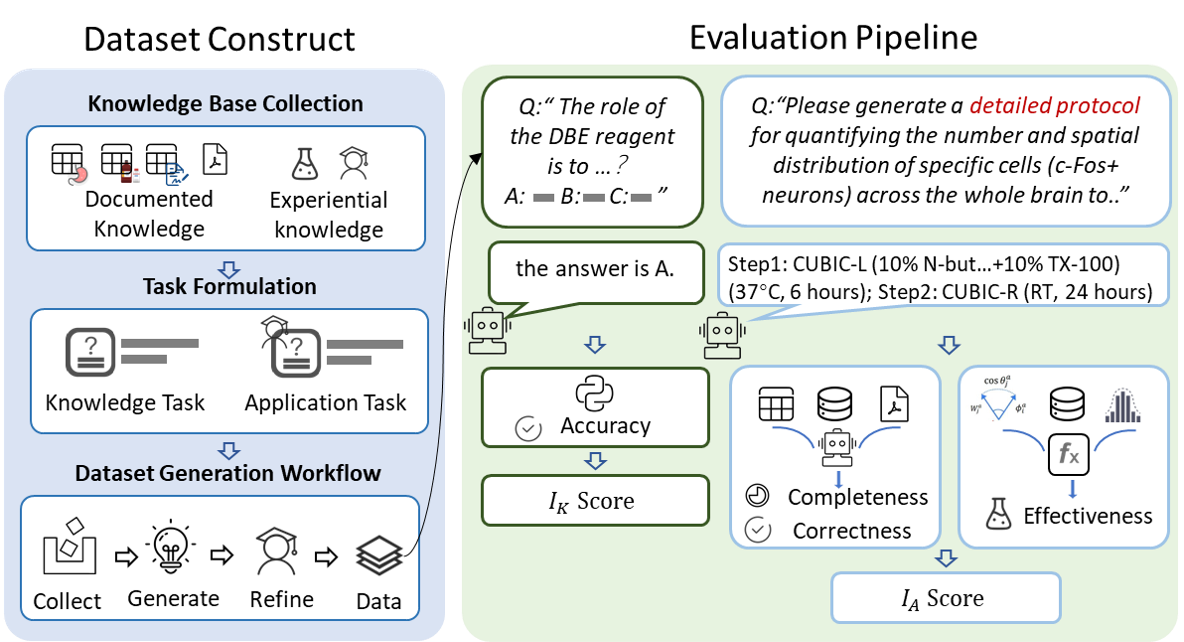
\includegraphics[width=0.8\textwidth]{figures/overview.png}
\caption{Overview of ClearEval. A TOC feasibility database is constructed
from wet-lab experimental records, curated literature chunks, and
expert-reviewed constraints. The database supports both task construction
and protocol scoring. The Knowledge track is scored by the Knowledge Index
($I_K$), while the Application track is scored by the Application Index
($I_A$), which combines Completeness, Correctness, and Effectiveness.}
\label{fig:overview}
\end{figure*}

Tissue Optical Clearing (TOC) renders biological tissues optically transparent
by reducing light scattering and refractive-index mismatch, enabling
non-destructive, high-resolution 3D imaging via light-sheet
microscopy~\cite{ueda2020tissue,chung2013clarity}. However, designing a TOC
protocol is not a single-answer task. Given a specimen, labeling target,
imaging goal, and laboratory constraint, experimenters must choose a feasible
combination of clearing method, labeling strategy, refractive-index condition,
incubation schedule, sample geometry, and operational constraints. Multiple
combinations may be acceptable, but one incompatibility---for example, a
quenched fluorophore, an unsuitable method for the sample scale, or an
unrealistic incubation time---can invalidate the protocol and irreversibly
damage the specimen.

Existing biomedical LLM benchmarks, including MedQA~\cite{jin2021disease},
MMLU~\cite{hendrycks2021mmlu}, and recent biomedical
extensions~\cite{zhang2025benchmarking,wang2025cardbiomedbench,feng2024mediq},
mainly evaluate knowledge retrieval, question answering, or text-based
reasoning. These settings measure whether models know biomedical facts, but
they do not directly test whether a generated wet-lab protocol is feasible
under experimental constraints. Likewise, semantic metrics such as
BLEU~\cite{papineni2002bleu} and general-purpose LLM
evaluators~\cite{liu2023geval,li2024survey} do not explicitly evaluate
method--label compatibility, refractive-index suitability, or timing
plausibility. This creates a gap between knowledge evaluation and
pre-experimental feasibility checking.

We introduce \textbf{ClearEval}, a database-grounded feasibility benchmark for
LLM-generated TOC protocols (Fig.~\ref{fig:overview}). ClearEval integrates 372 wet-lab experimental
records, 400+ curated tissue-clearing literature chunks, and expert-reviewed
TOC constraints into a structured feasibility database. This database supports
both task construction and protocol scoring. The benchmark contains 2{,}588
multiple-choice questions for static knowledge and 253 open-ended scenarios for
protocol generation. Generated protocols are evaluated by our
\textbf{CCE (Completeness, Correctness, Effectiveness)} framework, which
combines rubric-based procedural assessment with database-grounded rules and
formulas for experimental effectiveness.

Experiments on 13 state-of-the-art LLMs show that static knowledge performance
is uniformly high, whereas open-ended feasibility evaluation remains
discriminative. For example, GPT-5.2-Fast achieves 91.1\% on the Knowledge
Index but only 61.2 on the Application Index
(Table~\ref{tab:main_results_total}); MCQ profiles are tightly clustered, while
OEQ-based CCE scores expose model-specific execution failures. The most reliable failures arise from
executable parameterization, especially matching fluorescent markers to the
required labeling targets. Our contributions are: (1) a structured TOC feasibility database with
traceable wet-lab records, literature evidence, and expert-reviewed constraints;
(2) a database-grounded CCE checker that evaluates generated TOC protocols
through procedural completeness/correctness and deterministic feasibility checks,
without reference text or single-answer matching; (3) a TOC-specific finding
that current LLMs show a gap between static knowledge and executable parameter
binding, especially marker--target mismatch and method anchoring; and (4) a
controlled grounding probe showing that compact KB-RAG reduces marker--target
mismatch but exposes labeling--RI--timing trade-offs, motivating balanced
feasibility checking.



\section{Related Works}\label{sec:related}

\noindent\textbf{Scientific and biomedical LLM evaluation.}
The evaluation of scientific and biomedical LLMs has moved from general
knowledge tests toward more specialized biomedical and research-oriented tasks.
Benchmarks such as MMLU~\cite{hendrycks2021mmlu},
MedQA~\cite{jin2021disease}, Med-PaLM-style
evaluations~\cite{singhal2023medpalm}, and recent biomedical
benchmarks~\cite{zhang2025benchmarking,wang2025cardbiomedbench,feng2024mediq}
measure knowledge retrieval, clinical reasoning, biomedical NLP, and
interactive question answering. These resources provide standardized evidence
for biomedical competence, but their outputs are usually closed-form answers,
short explanations, or task-specific labels rather than executable wet-lab
protocols.

\noindent\textbf{Biological protocol and wet-lab benchmarks.}
Recent benchmarks have extended LLM evaluation toward biological protocols and
laboratory workflows. BioProBench~\cite{bioprobench} studies biological
protocol understanding and reasoning across multiple subfields, including
protocol QA, step ordering, error correction, generation, and reasoning.
LAB-Bench~\cite{labbench} evaluates language models on biology research tasks,
including literature use, protocol planning, and data analysis. BixBench
~\cite{bixbench} considers multi-step computational-biology agent tasks.
SeedBench~\cite{ying2025seedbench} similarly targets a single wet-lab subdomain
(seed science) but evaluates multi-task knowledge rather than parameter-level
protocol feasibility. These benchmarks characterize broad biological or research
capabilities. ClearEval
focuses on a complementary setting: parameter-level feasibility assessment for
LLM-generated Tissue Optical Clearing protocols, where multiple method--marker
--time combinations may be acceptable and must be checked against explicit
experimental constraints.

\noindent\textbf{Automatic evaluation, TOC, and pre-experimental checking.}
Automatic evaluation methods, including text-overlap metrics such as
BLEU~\cite{papineni2002bleu} and LLM-based evaluators such as
G-Eval~\cite{liu2023geval}, enable scalable assessment of generated outputs.
Recent work has also analyzed systematic effects in LLM-as-a-judge
methods~\cite{li2024survey,zheng2023judging}. In ClearEval, LLM judgment is
used for rubric-defined procedural dimensions, while Effectiveness is computed
from a structured TOC feasibility database. TOC methods (CLARITY, CUBIC, iDISCO,
uDISCO, PEGASOS) enable high-resolution 3D imaging across tissue and organ
scales~\cite{chung2013clarity,ueda2020tissue,wang2025advances,richardson2025unlocking,mai2024tissue};
ClearEval organizes this literature into a machine-readable feasibility checker
for LLM-generated protocols, a pre-experimental component for vertical
scientific agents~\cite{boiko2023autonomous,hartung2025ai}.




\section{The ClearEval Benchmark}\label{sec:benchmark}
ClearEval is organized around three linked components: a TOC feasibility
database, a dual-track task suite, and a scoring framework
(Fig.~\ref{fig:overview}). The feasibility database converts experimental
records, literature evidence, and expert-reviewed TOC constraints into
machine-readable resources. The task suite uses these resources to construct
knowledge questions and open-ended protocol-design scenarios. The scoring
framework evaluates model outputs with a Knowledge Index ($I_K$) for MCQs and
an Application Index ($I_A$) for generated protocols.

\subsection{TOC Feasibility Database}
ClearEval formalizes TOC protocol constraints as a structured feasibility
database. The database integrates 372 wet-lab experimental records used to
support clearing-time intervals, 400+ curated tissue-clearing literature
chunks, and expert-reviewed constraints on tissues, molecular targets,
fluorescent markers, clearing-method properties, refractive-index conditions,
sample scales, and compatibility rules. These resources are encoded into seven
machine-readable knowledge bases, with inventory, provenance, and review
status summarized in Table~\ref{tab:db_inventory} and fully documented in Appendix~\ref{app:curation}.

\begin{table}[htbp]
\centering
\caption{Feasibility database inventory: knowledge bases, content, provenance, and the Effectiveness sub-metric that reads from each.}
\label{tab:db_inventory}
\resizebox{\columnwidth}{!}{%
\begin{tabular}{l r l l}
\toprule
\textbf{Knowledge Base} & \textbf{Entries} & \textbf{Provenance} & \textbf{Metric} \\
\midrule
Method capability vectors & 20 methods, 6 axes & Expert review + literature & $S_{method}$ \\
Fluorophore compat.\ matrix & marker$\times$method & Expert review + literature & $S_{label}$ \\
Tissue \& target table & 30+ tissue types & Literature + expert & $S_{label}$ \\
RI references ($\sigma_{RI}$) & 18 clearing methods & Literature~\cite{ueda2020tissue,chung2013clarity} & $S_{trans}$ \\
Timing database ($\tau$) & 126 (method, tier) rows & 372 wet-lab records + lit. & $S_{time}$ \\
Wet-lab experimental records & 372 protocols & Lab data & Task + $S_{time}$ \\
Literature chunks & 400+ paragraphs & TOC literature & Task construction \\
\bottomrule
\end{tabular}%
}
\end{table}

The database is designed to support feasibility assessment rather than
single-answer protocol matching. For method selection, each clearing method is
represented along six experimental axes: fluorescence/protein preservation, dye
permeability, clearing capacity, sample geometry, operational economy, and
biosafety. These axes provide a shared constraint space for comparing the
requirements of an experimental scenario with the properties of candidate
clearing strategies.

\subsection{Task Suite Construction}
ClearEval contains two task tracks. The Knowledge track evaluates static TOC
knowledge. Expert-authored templates are instantiated against the feasibility
database through controlled-vocabulary substitution, producing 2{,}588
multiple-choice questions: 533 named-entity questions, 1{,}350
domain-knowledge questions, and 705 task-scenario questions. Each question uses an
8-option format, after deduplication and option shuffling. All reported $I_K$
values use a $768$-question development split ($30$ held out for validation).

The Application track evaluates open-ended TOC protocol generation. We define
60 expert-designed scientific missions across biological scales and combine
them with the feasibility database to construct constrained experimental
scenarios. These scenarios are further augmented with real wet-lab challenges
and quality-filtered to 253 open-ended tasks. Because TOC protocol design may
admit multiple feasible method--marker--time combinations, these tasks are not
graded by reference-text similarity. They are instead evaluated by the scoring
framework below.

\subsection{Scoring Framework}
ClearEval scores model outputs at two levels (Table~\ref{tab:metrics}). The
Knowledge Index ($I_K$) macro-averages accuracy within each of the three MCQ
super-categories (Tissue, Reagent, Method), then averages the three.
$I_K$ is not a protocol-feasibility score; it is a prerequisite knowledge audit
used to disambiguate whether application failures arise from missing TOC
knowledge or from failure to bind known constraints into executable protocol
parameters. The Application Index ($I_A$) evaluates open-ended generated
protocols through three dimensions: Completeness, Correctness, and
Effectiveness:
\begin{equation}
I_A = \min(\text{Completeness}, \text{Correctness}, \text{Effectiveness}).
\end{equation}
This bottleneck formulation reflects wet-lab practice: a protocol can be
detailed and fluent, yet still fail if one essential component is missing,
inconsistent, or experimentally infeasible. Thus, CCE denotes the scoring
structure of the Application track, whereas ClearEval as a whole combines both
static knowledge evaluation and application-level feasibility assessment.

\begin{table}[htbp]
\centering
\caption{The hierarchical metric system of ClearEval. Evaluation scales from
static knowledge retrieval to empirically grounded protocol execution. Within
each Application dimension, sub-scores are normalized to $[0,1]$ and combined by
the listed weights.}
\label{tab:metrics}
\resizebox{\columnwidth}{!}{
\begin{tabular}{l l l l c}
\toprule
\textbf{Level} & \textbf{Dimension} & \textbf{Sub-Metric} &
\textbf{Method} & \textbf{Weight} \\
\midrule
Knowledge ($I_K$) & Static Retrieval & Accuracy &
Deterministic & 100\% \\
\midrule
\multirow{10}{*}{Application ($I_A$)}
& \multirow{2}{*}{Completeness} & Step Integrity &
LLM-Judge & 40\% \\
& & Param Detail & LLM-Judge & 60\% \\
\cmidrule{2-5}
& \multirow{4}{*}{Correctness} & Seq. Logic ($co\_order$) &
LLM-Judge & 25\% \\
& & Method Consist. ($co\_method$) & LLM-Judge & 25\% \\
& & Param Consist. ($co\_param$) & LLM-Judge & 25\% \\
& & Chem. Safety ($co\_chem$) & LLM-Judge & 25\% \\
\cmidrule{2-5}
& \multirow{4}{*}{Effectiveness} & Method Suit. ($S_{method}$) &
Signed Fit & 25\% \\
& & Label Compat. ($S_{label}$) & Rule-Based & 25\% \\
& & Trans. Validity ($S_{trans}$) & Physics Eq. & 25\% \\
& & Time Efficiency ($S_{time}$) & Physics Eq. & 25\% \\
\midrule
\textbf{Overall} & Expert Score & Harmonic Mean &
Aggregation & 100\% \\
\bottomrule
\end{tabular}%
}
\end{table}

\paragraph{Completeness and Correctness.}
Completeness measures whether a protocol specifies a runnable TOC experiment,
via Step Integrity (are essential stages---fixation/pre-treatment, labeling,
clearing, RI matching, imaging preparation---present when applicable) and
Parameter Detail (are key parameters given: reagent/method choice, sample scale,
incubation time, temperature, concentration, labeling, imaging settings).
Correctness measures internal consistency with TOC principles through four
equally-weighted sub-checks: Sequential Logic ($co\_order$, plausible wet-lab
ordering); Method Consistency ($co\_method$, method matches goal and sample);
Parameter Consistency ($co\_param$, scale/timing/concentration/temperature
mutually consistent and respecting diffusion limits); and Chemical Safety
($co\_chem$, no introduced non-standard hazard). Both are scored by an LLM judge
(GPT-5.4) under a fixed rubric, since they require interpreting free-form text.

\paragraph{Effectiveness.}
Effectiveness evaluates whether the extracted experimental choices satisfy
TOC-specific feasibility constraints. Unlike Completeness and Correctness, it
is scored by deterministic, non-LLM checks that read from the TOC feasibility
database (Appendix~\ref{app:curation}). From each generated protocol, we
extract the clearing method, labeling target, fluorescent marker or labeling
strategy, refractive-index condition, and total processing time. These fields
are scored by four sub-metrics:
\begin{equation}
\text{Effectiveness}
= \tfrac{1}{4}\big(S_{method} + S_{label} + S_{trans} + S_{time}\big),
\end{equation}
where $S_{label},S_{trans},S_{time}\in[0,1]$ are normalized by their maxima
($6$, $3$, and $3$). Method suitability $S_{method}=(F_{method}+1)/2\in[0,1]$
is derived from the signed fit $F_{method}\in[-1,+1]$ (defined below):
$S_{method}{=}0.5$ is neutral; $S_{method}{<}0.5$ penalizes Effectiveness when
the chosen method conflicts with the scenario.

\noindent\textbf{Method suitability ($S_{method}$).}
Each clearing method carries a \emph{signed} six-dimensional capability vector:
five axes (fluorescent-protein preservation, dye penetration, geometry,
operational economy, safety) lie in $[-1,+1]$---a positive entry means the
method helps that objective, a negative entry that it actively harms it (an
organic solvent quenches endogenous fluorescence, $c_{\text{F\_fp}}<0$)---while
clearing power $c_{\text{C\_opt}}\in[0,1]$ is a non-negative magnitude. Each
scenario is associated with a frozen demand vector---generated from scenario
metadata during benchmark construction and expert-reviewed before model
evaluation---giving every axis a target $t_a\in[0,1]$ and a constraint weight
$w_a\in\{0,0.5,1\}$ ($w_a=0$ when the scenario is silent). No LLM is invoked
to infer the demand vector from model outputs during scoring. The per-axis
demand strength $d_a=w_a t_a$ makes unconstrained axes drop out. The two
labeling axes are mutually exclusive: whichever of FP-preservation /
dye-penetration has the larger weighted demand is emphasized ($\times2$) and the
other zeroed. The signed need-weighted fit is
\begin{equation}
F_{method}
= \frac{\sum_a d_a\, c_a}{\sum_a d_a}\ \in[-1,+1],
\end{equation}
positive when the method matches the scenario's binding constraints and negative
when it conflicts (e.g.\ an FP-quenching solvent for a reporter-line sample),
replacing an earlier cosine variant that collapsed onto a single default method.
The normalized method suitability $S_{method}=(F_{method}+1)/2\in[0,1]$ maps
full conflict ($F_{method}{=}{-1}$) to $S_{method}{=}0$ and full match
($F_{method}{=}1$) to $S_{method}{=}1$.

\noindent\textbf{Label compatibility ($S_{label}$, max $6$).}
This metric evaluates whether the proposed labeling strategy is compatible
with the biological target and the selected clearing method:
\begin{equation}
S_{label}
= \min(S_{target}, S_{marker}, S_{method\text{-}marker}).
\end{equation}
$S_{target}$ checks whether the marker matches the required labeling target;
$S_{marker}$ checks marker--fluorophore compatibility; and
$S_{method\text{-}marker}$ checks fluorophore compatibility with the selected
clearing method using the quenching matrix. Each term is scored on $[0,6]$.
The minimum operator implements a hard feasibility rule: failure of any one
check makes the labeling strategy unusable.

\noindent\textbf{Transparency validity ($S_{trans}$, max $3$).}
This metric evaluates whether the refractive-index condition associated with
the selected method is compatible with the tissue and sample scale. The score
penalizes the gap between the tissue reference RI ($RI_{tissue}$) and the
method RI ($RI_{ref}$) using a Gaussian tolerance $\sigma_{RI}$:
\begin{equation}
S_{trans}
= 3 \cdot
\exp\left(
-\frac{(RI_{tissue}-RI_{ref})^2}{2\sigma_{RI}^2}
\right).
\end{equation}
$S_{trans}$ is set to $0$ when the selected method has no supported entry for
the requested sample scale in the timing database.

\noindent\textbf{Time efficiency ($S_{time}$, max $3$).}
The proposed total processing time is compared with an evidence-supported
window $[t_{min},t_{max}]$. These windows are derived from TOC literature,
372 wet-lab experimental records, and expert review. Let $\Delta t$ denote the
deviation from this window, with $\Delta t=0$ when the proposed time falls
inside the interval. Out-of-window timing is penalized by
\begin{equation}
S_{time}
= 3 \cdot
\exp\left(
-\frac{\Delta t^2}{2\tau^2}
\right),
\end{equation}
where $\tau$ is set deterministically to $0.2\times$ the median clearing time.

All timing windows, RI references, and $\sigma_{RI}/\tau$ tolerances trace to
literature, wet-lab records, and expert review (Appendix~\ref{app:curation}).
Effectiveness is the clamped mean of the four normalized sub-scores, scaled to
$[0,100]$ before entering the $I_A$ bottleneck.

\paragraph{Overall Expert Score.}
The final ClearEval Expert Score combines static knowledge and
application-level feasibility using the harmonic mean:
\begin{equation}
\text{Score} = \frac{2 I_K I_A}{I_K + I_A}.
\end{equation}
This aggregation penalizes models that perform well on TOC knowledge questions
but fail to generate experimentally feasible protocols.

\section{Experiments}
\subsection{Models and Settings}
We benchmark 13 LLMs across the GPT, Gemini, Claude, DeepSeek, GLM, and Qwen
families. For all evaluated API models we set temperature to $0.0$ for both
Knowledge and Application tasks to maximize reproducibility; reasoning variants
additionally run in their native thinking mode.
Exact provider snapshot strings, context windows, maximum output tokens, and
API call dates are released in the repository configuration
(Appendix~\ref{app:repro}).

\subsection{Calibration of the Automated Metrics}\label{sec:calib}
Before reporting model rankings, we validate the automated CCE scores against
blinded expert consensus on 240 protocols (20 scenarios $\times$ 12 models).
Because Pearson correlation alone ignores absolute bias, we report, per
dimension, Pearson $r$, Spearman $\rho$, ICC(2,1), quadratic-weighted $\kappa$,
and Krippendorff's $\alpha$ (Table~\ref{tab:calib}; full 14-row sub-dimension
breakdown in Appendix~\ref{app:judge}). The aggregate CCE dimensions align well
with experts (ICC $0.75$/$0.74$/$0.69$ for Completeness/Correctness/Effectiveness;
Overall $r=0.79$). Agreement is \emph{uneven} across the Effectiveness sub-metrics.
Method suitability ($S_{method}$)---the signed need-weighted fit, validated
against expert method-suitability ratings we collected specifically---is among
the best-calibrated ($\mathrm{ICC}\,0.82$, $r{=}0.83$), confirming that the
signed axis space captures how experts judge method choice; timing ($S_{time}$,
ICC $0.78$) also tracks experts strongly and transparency ($S_{trans}$, $0.58$)
moderately. The exception is label compatibility ($S_{label}$, ICC $0.51$): its
hard-minimum over three binary checks is coarser than the graded expert scale,
so although it is the dominant execution \emph{failure} (Sec.~\ref{sec:diag}) it
is the most weakly-calibrated sub-metric. On the Correctness side all four
checks calibrate well, including chemical safety ($co\_chem$,
$\mathrm{ICC}\,0.80$) once its rubric was revised to flag only introduced
hazards---not the \emph{absence} of unrequested safety caveats---and re-judged
with GPT-5.4 ($28\%$ penalized).

\begin{table}[!t]
    \centering
    \caption{Agreement of automated vs.\ blinded expert-consensus scores on 240
    protocols (20 scenarios $\times$ 12 models). ICC${=}$ICC(2,1);
    QWK${=}$quadratic-weighted $\kappa$; $\alpha{=}$interval Krippendorff. Full
    14-row breakdown in Appendix~\ref{app:judge}.}
    \label{tab:calib}
    \resizebox{\columnwidth}{!}{%
    \begin{tabular}{l c c c c c}
        \toprule
        \textbf{Dimension} & \textbf{Pearson} $r$ & \textbf{Spearman} & \textbf{ICC} & \textbf{QWK} & $\boldsymbol{\alpha}$ \\
        \midrule
        Completeness  & 0.77 & 0.79 & 0.75 & 0.70 & 0.75 \\
        Correctness   & 0.79 & 0.77 & 0.74 & 0.72 & 0.73 \\
        Effectiveness & 0.71 & 0.72 & 0.69 & 0.68 & 0.69 \\
        Overall       & 0.79 & 0.79 & 0.74 & 0.73 & 0.74 \\
        \midrule
        \multicolumn{6}{l}{\textit{Effectiveness sub-metrics}} \\
        $S_{method}$ (method suit.) & 0.83 & 0.77 & 0.82 & 0.77 & 0.82 \\
        $S_{label}$ (rule)     & 0.51 & 0.48 & 0.51 & 0.51 & 0.51 \\
        $S_{trans}$ (physics)  & 0.63 & 0.46 & 0.58 & 0.52 & 0.56 \\
        $S_{time}$ (physics)   & 0.80 & 0.75 & 0.78 & 0.75 & 0.78 \\
        \bottomrule
    \end{tabular}%
    }
\end{table}

\subsection{Main Results: The Knowledge-Execution Gap}
On these calibrated metrics, Table~\ref{tab:main_results_total} reveals a stark
capability imbalance between
static recall and wet-lab execution: Knowledge indices cluster at $79$--$91$,
yet the bottleneck Application Index $I_A$ ranges from $62$ down to $35$. This is
visualized in Fig.~\ref{fig:radar_chart}: Knowledge proficiency is uniformly high
and tightly clustered, whereas Application performance is far more dispersed and
strongly model-dependent. Models
generally maintain
high procedural Completeness ($79$ on average) and Correctness ($69$), but are
weakest on Effectiveness ($56$ on average), the binding constraint for $9$ of the
$13$ models. The remaining four are limited by Correctness---Qwen3-235B,
Qwen3-32B, and Qwen3-14B, whose parameter- and method-consistency errors
pull Qwen3-14B to $35$---or by GLM-4.7-Think's truncated Completeness ($51$).
The dominant failure is label suitability ($S_{label}$): models
propose fluorescent markers that miss the scenario's required labeling targets
(Sec.~\ref{sec:diag}), exposing a severe knowledge--execution gap.

\begin{table*}[t]
    \centering
    \caption{Performance of state-of-the-art models on ClearEval. Evaluation
    covers Knowledge (MCQ) and Application (OEQ). $I_K$ represents the average
    of the Knowledge subset, $I_A$ represents the minimum score across the
    Application subset, and Total is their harmonic mean. GLM-4.7-Think's thinking-mode reasoning frequently
    exhausts the output-token budget and truncates its protocols, lowering its
    Completeness. $^\dagger$GLM-4.7-Think is not covered by the expert
    calibration (Sec.~\ref{sec:calib}); $^\ddagger$Gemini-3-Flash is scored on
    $251/253$ scenarios (two unparseable responses omitted, not a systematic
    filter).}
    \label{tab:main_results_total}
    \setlength{\tabcolsep}{4pt}
    \resizebox{0.74\textwidth}{!}{%
    \begin{tabular}{l cccc cccc c}
        \toprule
        \multirow{2}{*}{\textbf{Models}} & \multicolumn{4}{c}{\textbf{Knowledge (MCQ)}} & \multicolumn{4}{c}{\textbf{Application (OEQ)}} & \multirow{2}{*}{\textbf{Total}} \\
        \cmidrule(lr){2-5} \cmidrule(lr){6-9}
        & Tissue & Reagent & Method & $I_K$ & Com. & Cor. & Eff. & $I_A$ & \\
        \midrule
        \multicolumn{10}{l}{\textit{Proprietary Models}} \\
        \midrule
        GPT-5.2-Fast & \textbf{91.1} & \textbf{88.7} & 93.5 & \textbf{91.1} & \underline{97.0} & 84.4 & \underline{61.2} & \underline{61.2} & \textbf{73.2} \\
        GPT-5.2-Think & \underline{90.5} & \underline{87.3} & \underline{93.6} & \underline{90.5} & 96.9 & \textbf{85.4} & 60.5 & 60.5 & 72.5 \\
        Gemini-3-Flash$^\ddagger$ & 78.7 & 81.8 & 91.1 & 83.8 & 78.2 & 79.7 & 59.1 & 59.1 & 69.3 \\
        Gemini-3-Pro & 88.8 & 77.2 & 86.7 & 84.2 & 83.8 & \underline{85.0} & 53.1 & 53.1 & 65.1 \\
        Claude-4.6-Sonnet & 87.6 & 82.9 & \textbf{94.9} & 88.5 & \textbf{98.6} & 77.4 & \textbf{62.3} & \textbf{62.3} & \underline{73.1} \\
        \midrule
        \multicolumn{10}{l}{\textit{Open-Weight Models}} \\
        \midrule
        GLM-4.7 & 79.3 & 80.2 & 93.5 & 84.3 & 77.5 & 73.2 & 60.6 & 60.6 & 70.6 \\
        GLM-4.7-Think$^\dagger$ & 78.7 & 70.5 & 90.7 & 80.0 & 51.1 & 67.2 & 54.2 & 51.1 & 62.3 \\
        DeepSeek-V3.2 & 79.9 & 77.9 & 91.7 & 83.1 & 78.6 & 68.3 & 49.3 & 49.3 & 61.9 \\
        DeepSeek-V3.2-Think & 85.3 & 83.8 & 93.5 & 87.5 & 78.2 & 67.6 & 49.0 & 49.0 & 62.9 \\
        Qwen3-Max & 79.9 & \underline{87.3} & 93.1 & 86.8 & 87.0 & 72.5 & 60.9 & 60.9 & 71.6 \\
        Qwen3-235B-A22B & 77.5 & 81.2 & 89.1 & 82.6 & 76.8 & 52.4 & 56.4 & 52.4 & 64.1 \\
        Qwen3-32B & 73.4 & 78.6 & 89.9 & 80.6 & 61.7 & 50.8 & 51.3 & 50.8 & 62.3 \\
        Qwen3-14B & 73.4 & 77.8 & 88.4 & 79.9 & 58.4 & 35.3 & 53.5 & 35.3 & 48.9 \\
        \bottomrule
    \end{tabular}%
    }
\end{table*}

\begin{figure*}[t]
    \centering
    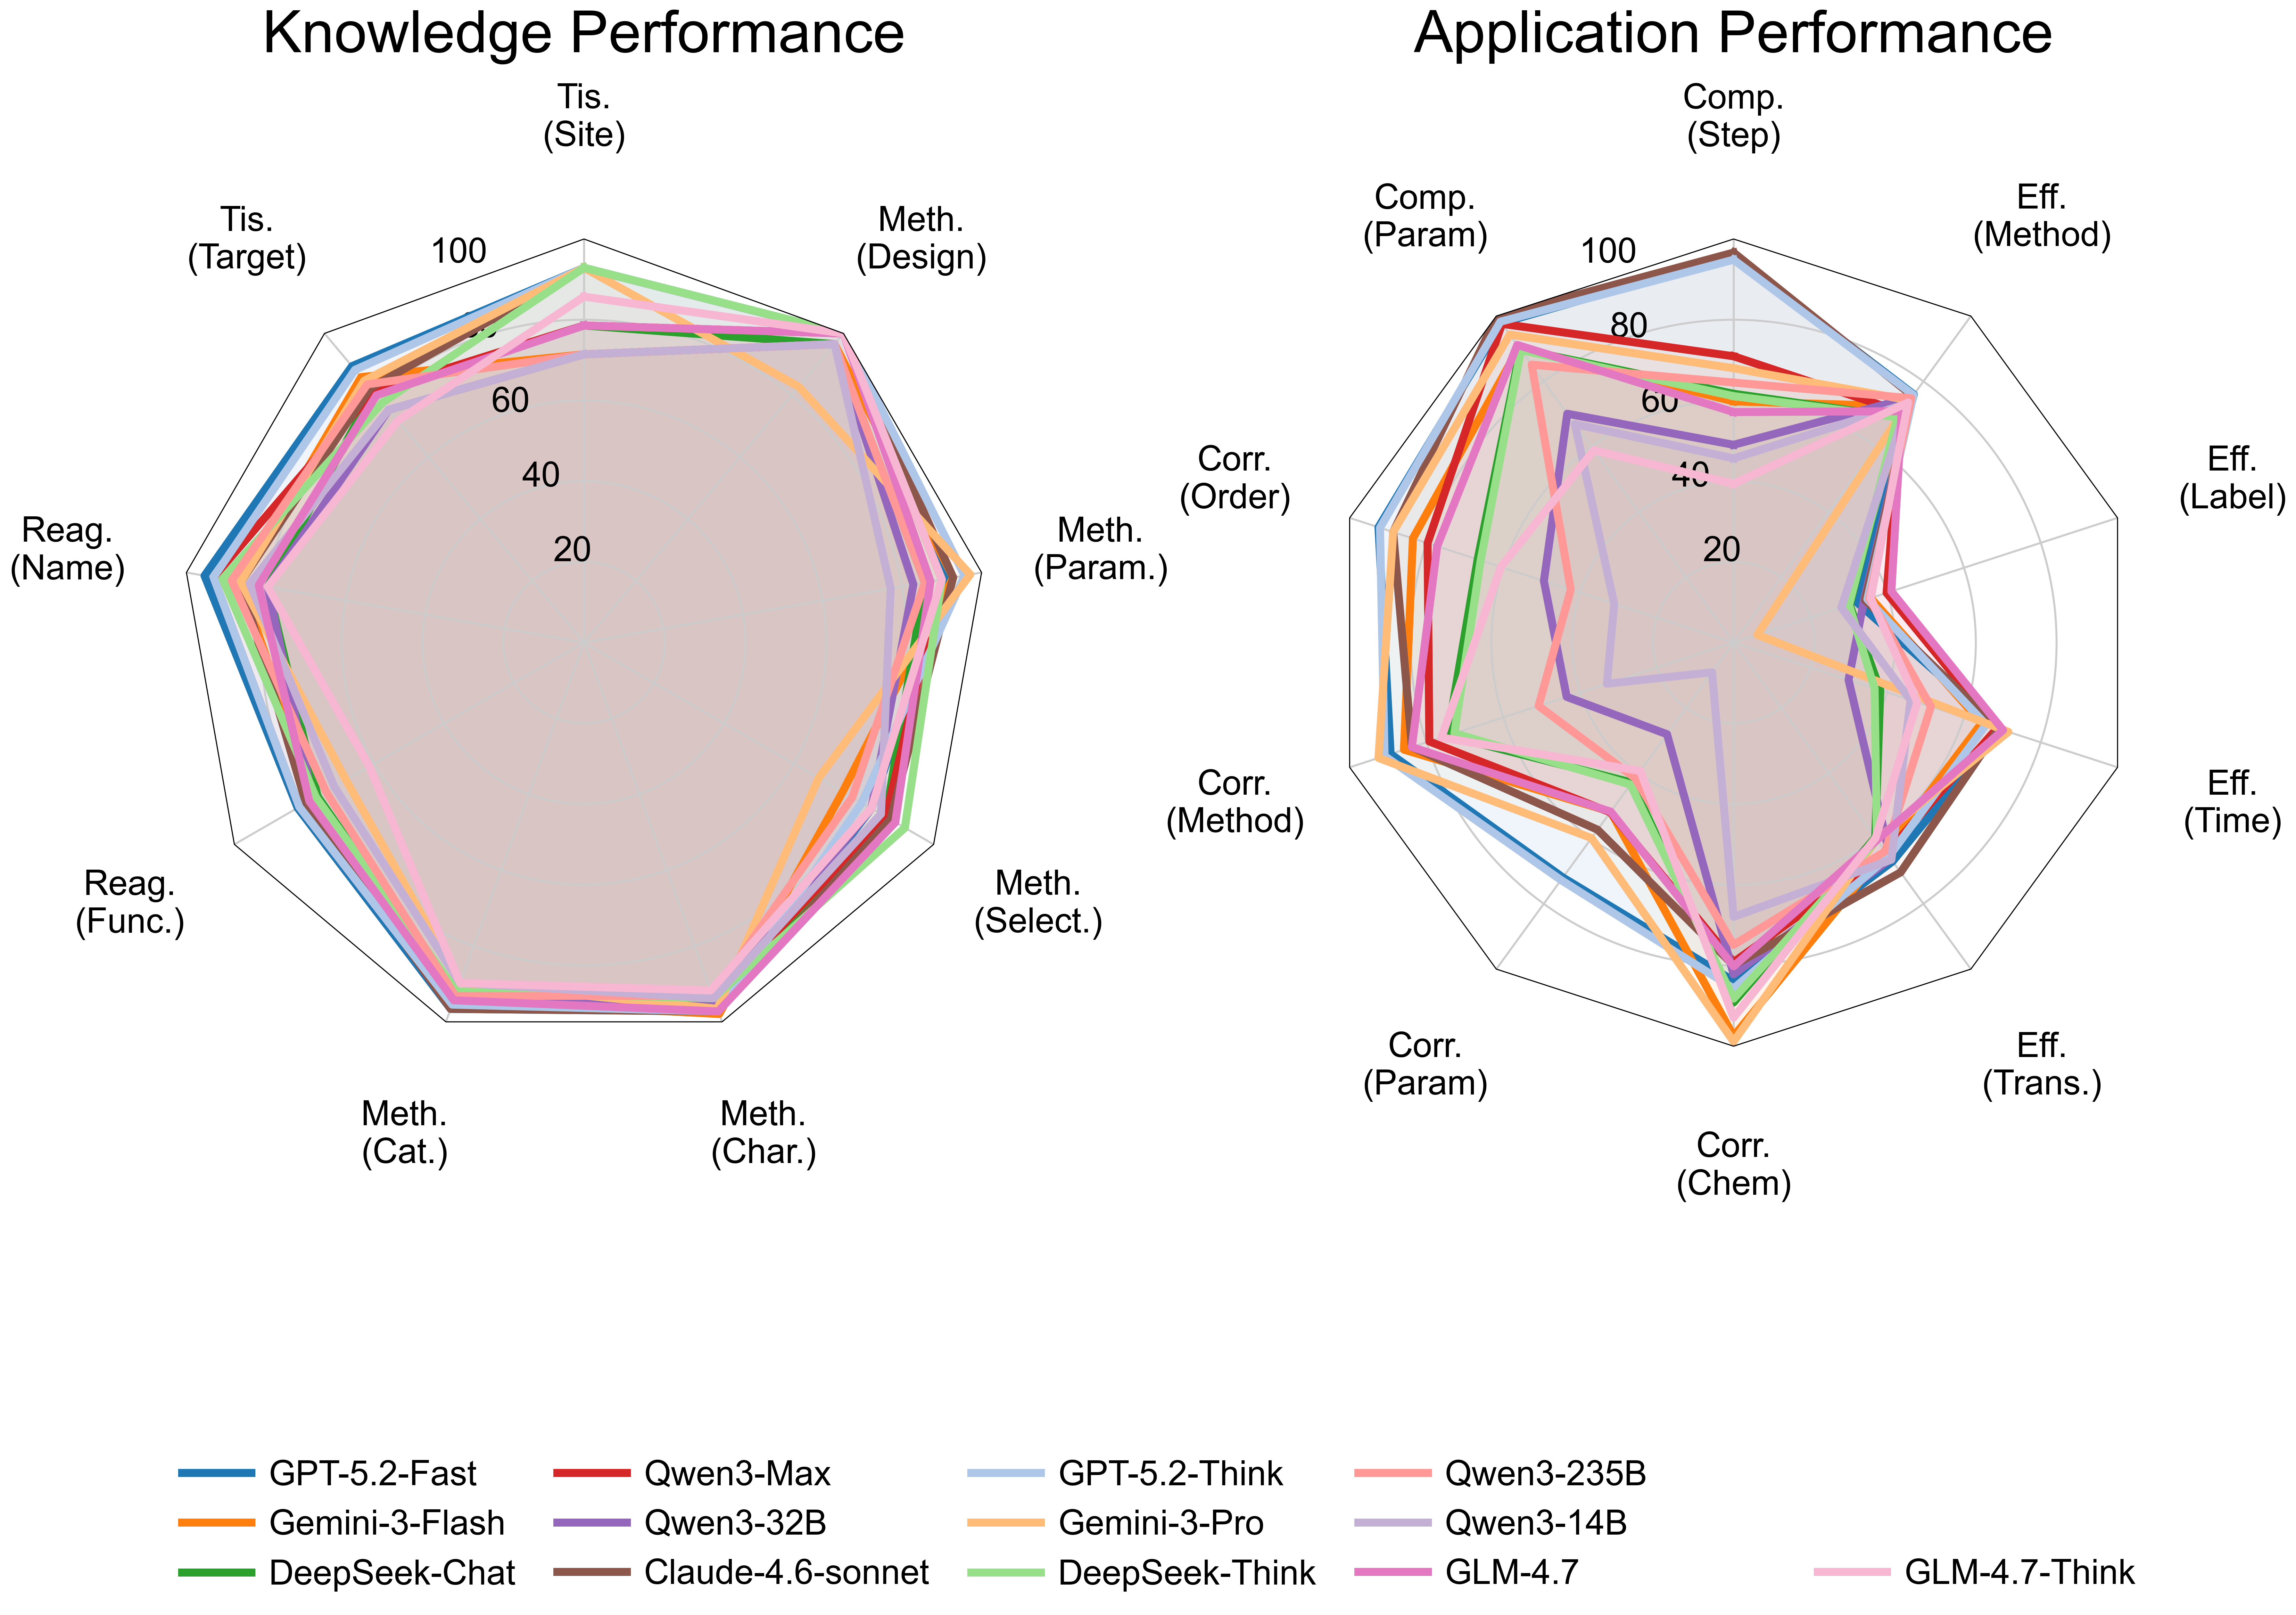
\includegraphics[width=0.62\textwidth]{figures/radar_chart.png}
    \caption{Performance comparison of 13 LLMs on ClearEval. Left: Knowledge
    Performance ($I_K$) across domain attributes (Tissue, Reagent, Method).
    Right: Application Performance ($I_A$), across the CCE sub-metrics. MCQ
    profiles are tightly clustered; CCE scores are far more dispersed and model-dependent.}
    \label{fig:radar_chart}
\end{figure*}

\subsection{Fine-Grained Diagnosis: Where Execution Fails}\label{sec:diag}
Averaging normalized sub-scores over all 253 scenarios and 13 models, the
\emph{reliably}-measured deficit concentrates in label suitability
(Fig.~\ref{fig:violin_limits}). \textbf{Label suitability} ($S_{label}$, mean
$0.32$) is a hard minimum over a marker--target match and two
fluorophore-compatibility checks, and $53\%$ of protocols score $0$. Decomposing
these zeros from the scorer's own breakdown shows the binding cause is
\textbf{marker--target mismatch}---the fluorescent markers models propose do not
match the scenario's required labeling targets. Of the $S_{label}{=}0$ cases,
$86\%$ are marker--target mismatches and the remaining $\sim$14\% are
fluorophore-compatibility failures; the quenching check binds in $\sim$41\% of
protocols, staying high on average ($4.2/6$) and zeroing in $\sim$10\%. The
marker--target zeros are \emph{deterministic} labeling
errors---directly verifiable, not scoring artifacts---so despite $S_{label}$'s
only moderate graded calibration (ICC $0.51$, Sec.~\ref{sec:calib}) this dominant
deficit is a trustworthy execution failure. The re-judged $co\_chem$ (GPT-5.4) flags
introduced hazards in $\sim$28\% of protocols.
Transparency ($S_{trans}$, $0.64$) and timing ($S_{time}$, $0.56$) are
moderately impaired, with small-sample timing failures: models over-estimate
clearing time (e.g.\ $\sim$10\,h for a $\leq 500\,\mu$m slice cleared in
$<2$\,h) against the refined windows.
$S_{time}$ stays well-calibrated (ICC $0.78$). Method suitability
($S_{method}$, $0.73$, ICC $0.82$) is comparatively high, so method
\emph{choice} is not the main deficit; the most reliable constraint these LLMs
miss is matching fluorescent markers to required targets.

\begin{figure}[!htb]
    \centering
    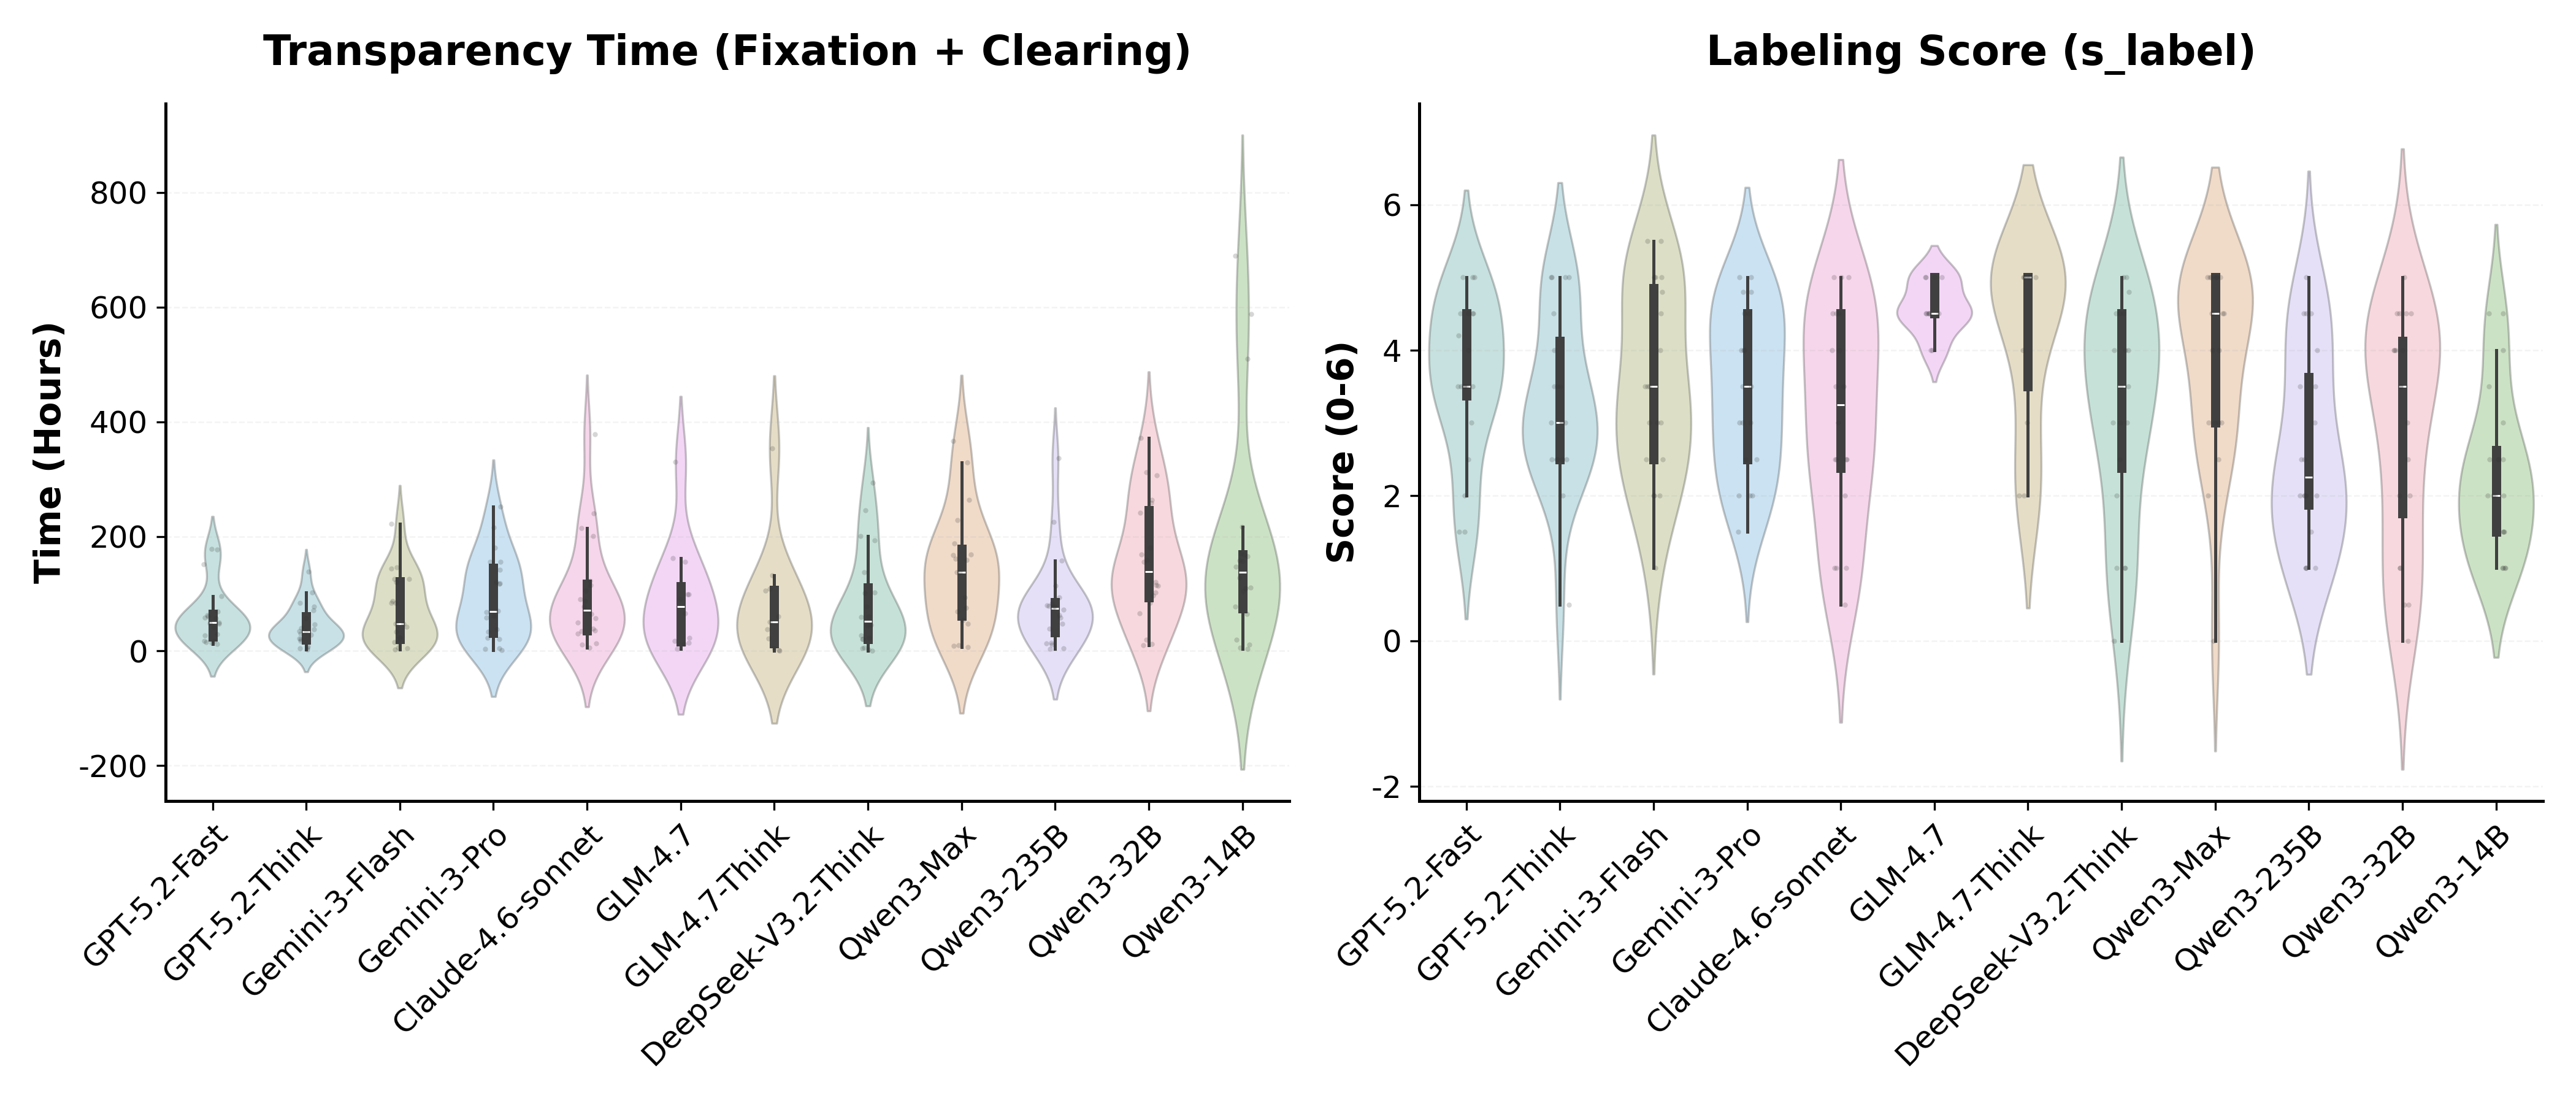
\includegraphics[width=\columnwidth]{figures/violin_plots.png}
    \caption{Effectiveness sub-metric distributions over all $3{,}287$
    protocols, normalized to $[0,1]$ (mean $\Diamond$, median $\circ$, IQR bar;
    $S_{method}{=}(F_{method}+1)/2$ so $0.5$ is neutral). $S_{label}$ ($0.32$) is
    the dominant failure; $S_{method}$ ($0.73$) is high and well-calibrated (ICC $0.82$).}
    \label{fig:violin_limits}
\end{figure}

\noindent\textbf{Method path-dependence.} Method \emph{selection} is
concentrated and largely scenario-independent (Fig.~\ref{fig:method_usage}):
iDISCO+ alone accounts for $43\%$ of all $3{,}287$ choices, and anchoring tracks
scale (entropy $1.35$--$2.97$ bits). Yet this is benign for suitability---iDISCO+
is broadly applicable (mean $S_{method}{=}0.78$, conflicting in $7\%$ of uses),
so the most anchored model (Qwen3-14B, $74\%$ iDISCO+) matches the most diverse
on $S_{method}$: the metric captures method \emph{conflict}, not per-scenario
reasoning. The same familiarity prior is instead harmful for
labeling---canonical fluorophores that miss the target (the $S_{label}$
collapse)---so its cost surfaces in labeling, not method choice.

\begin{figure}[!htb]
    \centering
    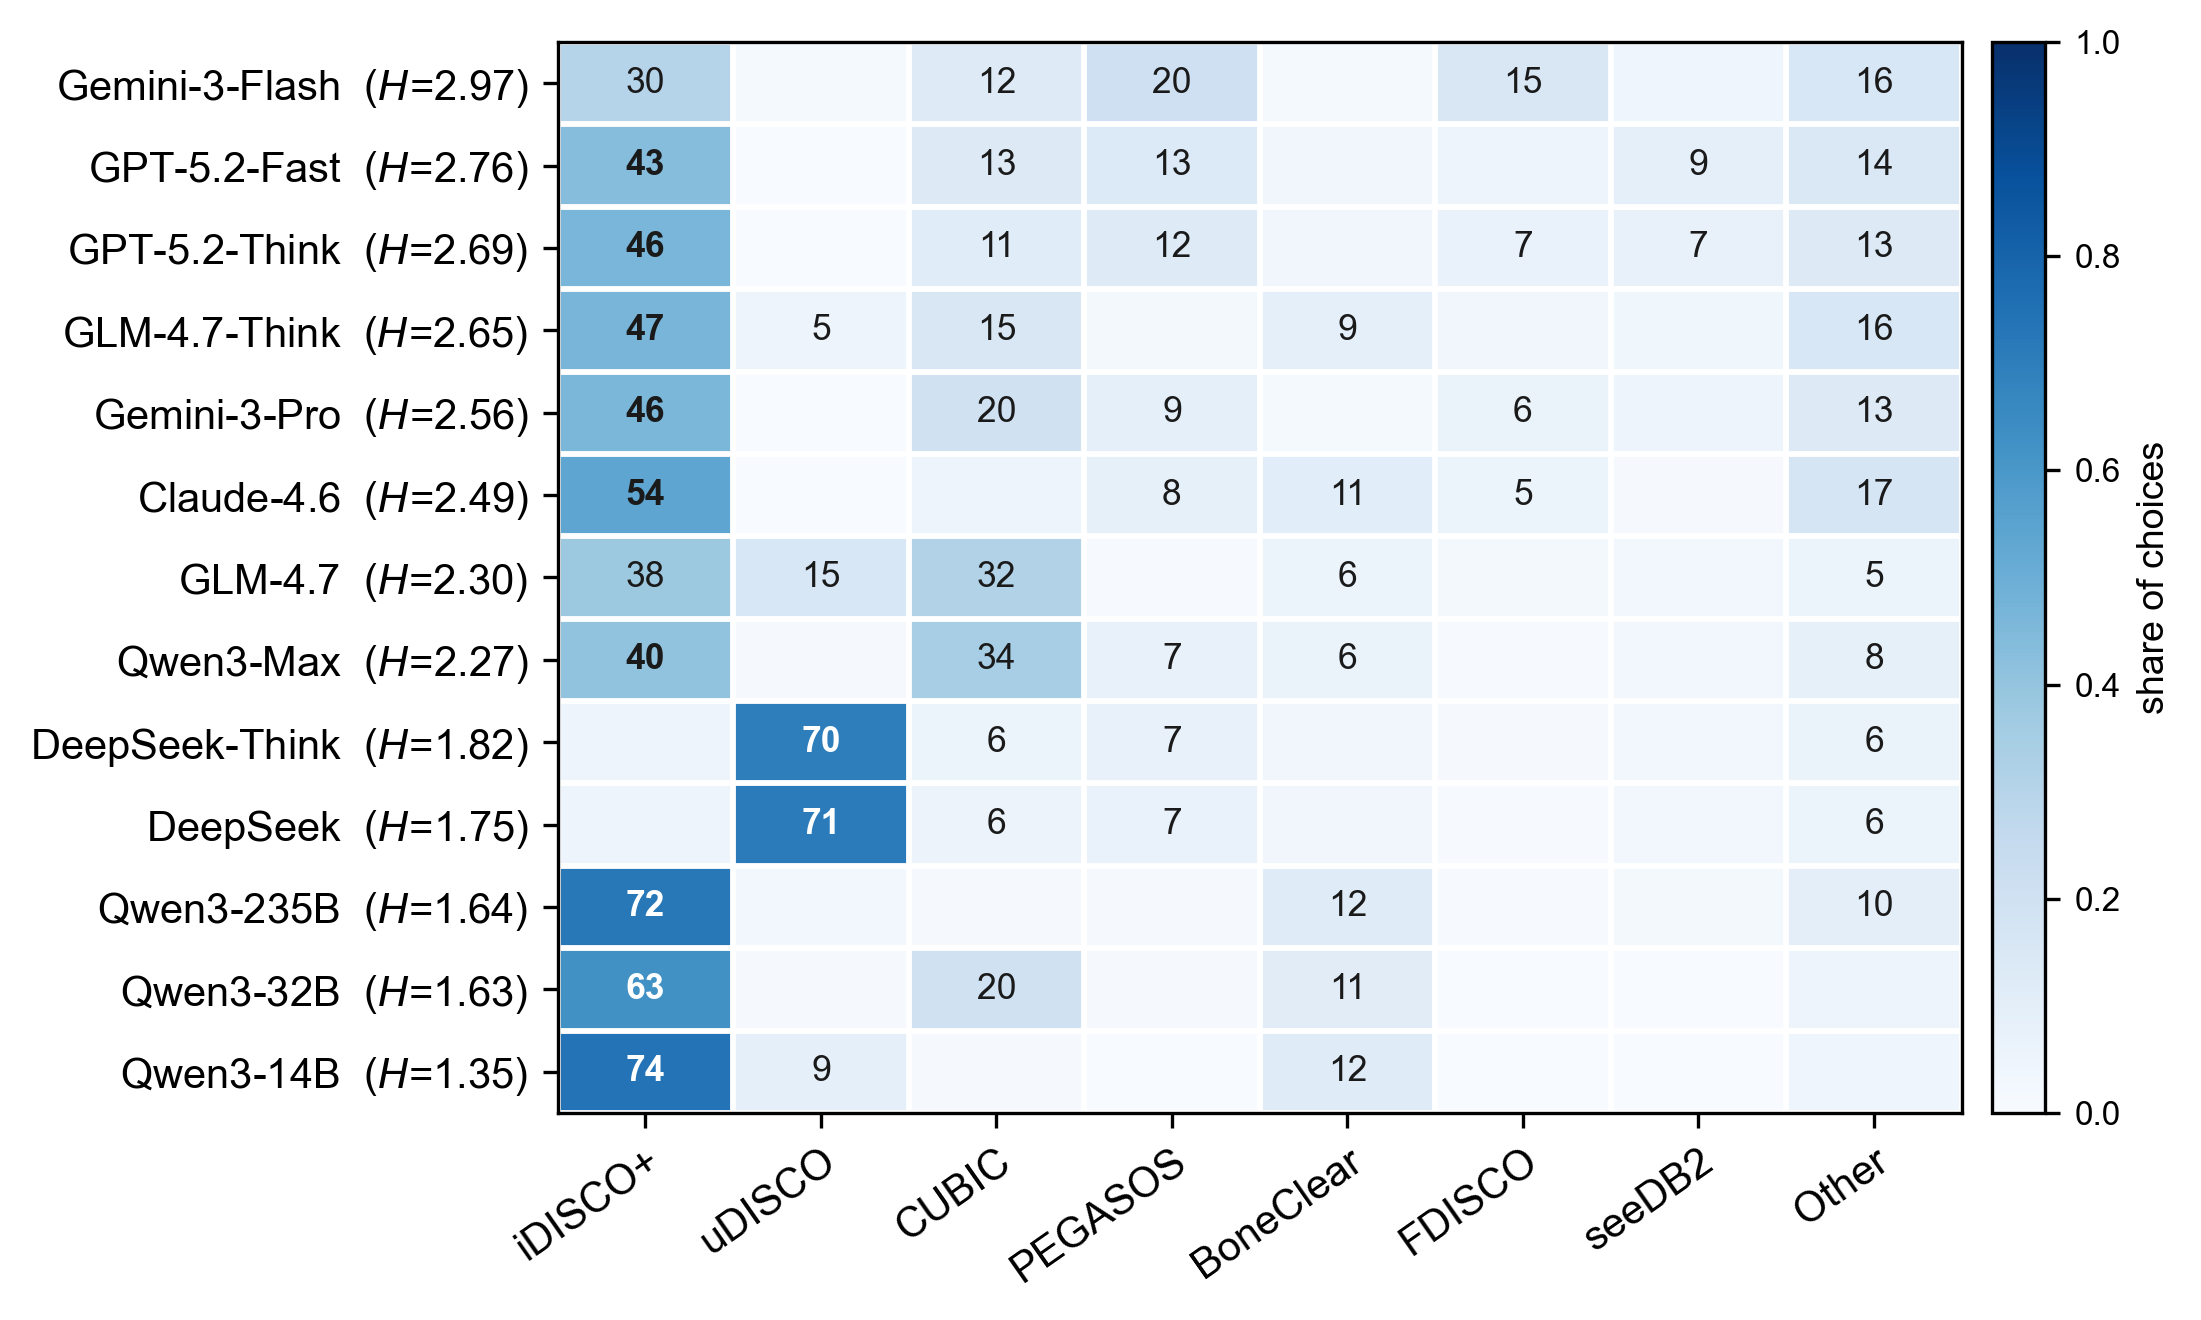
\includegraphics[width=\columnwidth]{figures/method_usage.png}
    \caption{Clearing-method selection per model (\% of choices), rows sorted by
    choice entropy $H$. iDISCO+ dominates ($43\%$); smaller models anchor hardest
    (Qwen3-14B $74\%$), DeepSeek on uDISCO---a strong default bias.}
    \label{fig:method_usage}
\end{figure}

\subsection{Inference-Time Robustness Protocol}\label{sec:baselines}
A natural follow-up is whether the knowledge--execution gap narrows once standard
inference-time grounding is applied, rather than being an artifact of greedy
decoding. We release a turnkey harness that scores grounding recipes against the
greedy default on the full 253-scenario Application set, and instantiate it on
three models spanning the capability range---GPT-5.2-Fast, Qwen3-Max, and
Qwen3-14B---across three settings: the
$1$-shot default; $+$\textbf{KB-RAG}, which prepends a per-scenario knowledge-base
context (standardized scenario slots, target$\rightarrow$marker candidate sets, and
qualitative method / compatibility records, \emph{with numeric RI/time targets and
gold protocols withheld so the answer key is never leaked}); and
$+$\textbf{KB-RAG$+$self-check}, a deliberately cheap alternative to
self-consistency in which the model runs one fixed feasibility checklist over its
grounded answer and revises exactly once. The per-scenario RAG context is built
deterministically from scenario metadata (identical across models) and released.
Every setting is scored by the same calibrated CCE pipeline (Sec.~\ref{sec:calib}),
so the bottleneck $I_A$ is directly comparable to
Table~\ref{tab:main_results_total}. This experiment is a controlled grounding probe
rather than an exhaustive prompting or agent benchmark; full literature-RAG and
agentic optimization are left to future work.

\begin{table*}[!t]
\centering
\small
\setlength{\tabcolsep}{5pt}
\caption{Inference-time grounding for three models (253 Application scenarios,
calibrated CCE pipeline). Com/Cor/Eff/$I_A$: percentages; sub-scores: normalized
$[0,1]$ means ($S_{method}{=}(F_{method}+1)/2$; others natively in $[0,1]$).
KB-RAG withholds numeric RI/time keys; SC is a single checklist revision.}
\label{tab:inference_time}
\begin{tabular}{llcccc cccc}
\toprule
Model & Setting & Com & Cor & Eff & $I_A$ & $S_{m}$ & $S_{lab}$ & $S_{tr}$ & $S_{ti}$ \\
\midrule
\multirow{3}{*}{GPT-5.2-Fast}
 & $1$-shot       & 97.0 & 84.4 & 61.2 & 61.2 & 0.76 & 0.32 & 0.67 & 0.70 \\
 & $+$KB-RAG      & 94.2 & 79.0 & 62.3 & 62.3 & 0.79 & 0.45 & 0.67 & 0.57 \\
 & $+$KB-RAG$+$SC & 92.0 & 80.2 & 63.2 & \textbf{63.2} & 0.79 & 0.60 & 0.60 & 0.54 \\
\midrule
\multirow{3}{*}{Qwen3-Max}
 & $1$-shot       & 87.0 & 72.5 & 60.9 & \textbf{60.9} & 0.71 & 0.40 & 0.64 & 0.69 \\
 & $+$KB-RAG      & 85.1 & 73.4 & 57.8 & 57.8 & 0.77 & 0.50 & 0.56 & 0.49 \\
 & $+$KB-RAG$+$SC & 85.2 & 73.6 & 58.6 & 58.6 & 0.76 & 0.56 & 0.57 & 0.45 \\
\midrule
\multirow{3}{*}{Qwen3-14B}
 & $1$-shot       & 58.4 & 35.3 & 53.5 & 35.3 & 0.73 & 0.28 & 0.66 & 0.46 \\
 & $+$KB-RAG      & 63.1 & 41.8 & 59.8 & 41.8 & 0.73 & 0.52 & 0.66 & 0.48 \\
 & $+$KB-RAG$+$SC & 63.3 & 42.4 & 60.6 & \textbf{42.4} & 0.73 & 0.55 & 0.66 & 0.49 \\
\bottomrule
\end{tabular}
\end{table*}

Grounding attacks the dominant failure mode: $S_{label}$ rises sharply for all
three models (GPT-5.2-Fast $0.32\!\rightarrow\!0.60$, Qwen3-Max
$0.40\!\rightarrow\!0.56$, Qwen3-14B $0.28\!\rightarrow\!0.55$), confirming
marker--target mismatch is an addressable knowledge gap. The $I_A$ gain is
model-dependent and largest where baseline execution is weakest: KB-RAG$+$SC lifts
Qwen3-14B by $+7.1$ ($35.3\!\rightarrow\!42.4$) and GPT-5.2-Fast by $+2.0$
($61.2\!\rightarrow\!63.2$), but slightly \emph{lowers} Qwen3-Max ($-2.3$):
grounding shifts selection toward organic solvents whose clearing times fit the
feasibility windows less tightly on soft tissue, and for Qwen3-Max this
transparency--time trade-off outweighs the label gain. Self-check is never worse
than KB-RAG alone; closing the marker--target gap is the primary lever.

\noindent\textbf{Retrieval/prompt variants do not lift all axes jointly.} We probed
three grounding-context designs---demand-ranked candidate methods (above),
refractive-index-family-aware ranking, and RI-aware ranking augmented with
per-method qualitative timing hints. Each improved a \emph{different subset} of the
effectiveness sub-scores, but none raised all four together: labeling ($S_{label}$)
improved under every variant, whereas RI-family-aware retrieval recovered
transparency validity ($S_{trans}$) without a net $I_A$ gain, as the induced shift
in method choice and stated timing offset it. That a single released,
non-per-model-tuned context trades one effectiveness axis for another is the
expected signature of a multi-constraint feasibility objective---not a mis-written
prompt---so jointly grounding method, marker, RI, and timing (with agentic
re-optimization) is left to future work.

\section{Discussion and Limitations}\label{sec:discussion}
Within TOC, ClearEval shows the bottleneck is not declarative retrieval but
executable parameterization---most reliably, matching fluorescent markers to the
required labeling targets, with refractive-index and timing errors
secondary. Whether this pattern generalizes across wet-lab subdomains is an open
question our single-subdomain design cannot settle.

\noindent\textbf{Scope and complementarity.} ClearEval covers one subdomain
(TOC); claims are about TOC feasibility, not general LLM scientific competence.
Generalizing requires re-curating subdomain-specific knowledge bases
(Appendix~\ref{app:curation}); we offer CCE as a transferable recipe.
Depth-first ClearEval and breadth-first benchmarks such as
BioProBench~\cite{bioprobench} are complementary, the former providing
parameter-level feasibility scoring, the latter broad coverage.

\noindent\textbf{Limitations.} ClearEval remains a static paradigm: real-world
wet labs involve stochastic variables (reagent degradation, tissue
heterogeneity) hard to model in silico, and our expert grounding is
literature-bounded rather than exhaustively re-measured. Future work should
integrate dynamic hardware feedback so agents iteratively optimize protocols
from real-time signals.

\section{Conclusion}
We presented ClearEval, an expert-curated benchmark for TOC protocol design
that shifts evaluation from semantic similarity to empirically grounded
functional validation. By leveraging a dual-track pipeline and a data-driven
CCE framework, ClearEval exposes a significant knowledge-execution gap in
current LLMs on TOC protocol design. Models excel at knowledge recall but
struggle with the marker--target matching and physical-feasibility constraints
required for wet-lab execution. ClearEval and the transferable CCE recipe aim to
facilitate reliable scientific agents, starting with tissue-clearing workflows.

\appendices

\section{Knowledge-Base Curation and Expert Grounding}\label{app:curation}
\noindent\textbf{Expert panel and consensus.} The knowledge bases and CCE
rubric were curated by a panel of tissue-clearing wet-lab experts with a
knowledge-graph specialist. Application protocols were scored blind against the
rubric then reconciled by consensus; released scores are per-protocol consensus
values.

\noindent\textbf{Knowledge bases and provenance.} Seven JSON knowledge bases
(listed in Table~\ref{tab:db_inventory}) ground the Effectiveness sub-metrics.
Each timing row carries a literature source key, URL, evidence locator, and
confidence level, providing a parameter-to-source audit trail. Timing tolerances
are derived deterministically as $\tau{=}0.2\times$ the median clearing time and
refined by expert review.

\noindent\textbf{Operationalization.} The Effectiveness terms read directly from
these bases: $S_{method}$ from the signed method-capability and
scenario-demand vectors (a signed need-weighted fit);
$S_{label}$ from the fluorophore-compatibility matrix (hard zero on quenching);
$S_{trans}$ from RI references and $\sigma_{RI}$, gated to zero when a (method,
tier) pair is unsupported; and $S_{time}$ from $[t_{min},t_{max}]$ and $\tau$.

\section{Judge Calibration Details}\label{app:judge}
Table~\ref{tab:calibfull} reports the full per-sub-dimension agreement between
automated and blinded expert-consensus scores ($n{=}240$), including the
now well-calibrated $S_{method}$. The two LLM-judged
dimensions use a fixed rubric (\texttt{eval\_oeq\_teacher\_rubric.txt},
\texttt{eval\_completeness\_checklist.txt}, released in the repository) at
temperature $0.0$. Because raw per-annotator sheets were not preserved, we report
expert-consensus-vs-automated agreement rather than human--human inter-annotator
reliability.

\begin{table}[htbp]
    \centering
    \caption{Full per-dimension agreement of automated vs.\ expert-consensus
    scores ($n{=}240$). ICC${=}$ICC(2,1); QWK${=}$quadratic-weighted $\kappa$;
    $\alpha{=}$interval Krippendorff.}
    \label{tab:calibfull}
    \small
    \begin{tabular}{l c c c c c}
        \toprule
        \textbf{Dimension} & $r$ & $\rho$ & \textbf{ICC} & \textbf{QWK} & $\boldsymbol{\alpha}$ \\
        \midrule
        $c\_step$  & 0.71 & 0.72 & 0.70 & 0.54 & 0.70 \\
        $c\_param$ & 0.71 & 0.71 & 0.68 & 0.60 & 0.67 \\
        \textbf{Completeness} & 0.77 & 0.79 & 0.75 & 0.70 & 0.75 \\
        \midrule
        $co\_order$  & 0.66 & 0.65 & 0.61 & 0.58 & 0.60 \\
        $co\_method$ & 0.83 & 0.81 & 0.79 & 0.77 & 0.79 \\
        $co\_param$  & 0.55 & 0.56 & 0.53 & 0.48 & 0.53 \\
        $co\_chem$   & 0.83 & 0.69 & 0.80 & 0.66 & 0.79 \\
        \textbf{Correctness} & 0.79 & 0.77 & 0.74 & 0.72 & 0.73 \\
        \midrule
        $S_{method}$ ($=\!(F_{method}\!+\!1)/2$) & 0.83 & 0.77 & 0.82 & 0.77 & 0.82 \\
        $S_{label}$  & 0.51 & 0.48 & 0.51 & 0.51 & 0.51 \\
        $S_{trans}$  & 0.63 & 0.46 & 0.58 & 0.52 & 0.56 \\
        $S_{time}$   & 0.80 & 0.75 & 0.78 & 0.75 & 0.78 \\
        \textbf{Effectiveness} & 0.71 & 0.72 & 0.69 & 0.68 & 0.69 \\
        \midrule
        \textbf{Overall} & 0.79 & 0.79 & 0.74 & 0.73 & 0.74 \\
        \bottomrule
    \end{tabular}
\end{table}

\section{Reproducibility and Artifact Manifest}\label{app:repro}
\noindent\textbf{Artifacts and determinism.} The repository releases the 253
Application scenarios and 2{,}588 MCQs, the seven knowledge bases, all 13 model
generations and their evaluation results, the generation/judge prompts, and the
scoring/plotting code (English README, \texttt{requirements.txt}). All evaluated
API models run at temperature $0.0$; since hosted
models are non-deterministic and snapshot aliases drift, we release the raw
responses---with provider snapshots and API-call dates---so results are
replayable even when regeneration is not bit-identical.

\noindent\textbf{Inference-time protocol (Sec.~\ref{sec:baselines}).} KB-RAG
prepends per-scenario cards---scenario slots, target$\rightarrow$marker candidate
sets, and qualitative method/compatibility records---built deterministically from
scenario metadata, with numeric RI/time targets and gold protocols withheld;
self-check runs one fixed feasibility checklist over the grounded answer and
revises exactly once (a cheap alternative to $k{=}5$ self-consistency). The
released harness also exposes few-shot and self-consistency recipes; the
single-model GPT-5.2-Fast instantiation is reported in
Table~\ref{tab:inference_time}.

% ---- Bibliography ----
\bibliographystyle{IEEEtran}
\bibliography{references}

\end{document}
